\documentclass[11pt,a4paper]{article}

% ============================================================
%  Rapport de projet pratique
%  Reconnaissance de plaques mineralogiques burkinabe
%  Cours : Reconnaissance de motifs --- IBAM / UJKZ
% ============================================================

\usepackage{fontspec}
\setmainfont{Latin Modern Roman}
\setsansfont{Latin Modern Sans}
\setmonofont{Latin Modern Mono}

\usepackage[french]{babel}

\usepackage{geometry}
\geometry{a4paper,top=2.5cm,bottom=2.5cm,left=2.5cm,right=2.5cm}

\usepackage{amsmath,amssymb}
\usepackage{xcolor}

% --- Numerotation I. / 1. / a. (pas de "chapitre"), tout en noir ---
\usepackage{titlesec}
\renewcommand{\thesection}{\Roman{section}}
\renewcommand{\thesubsection}{\arabic{subsection}}
\renewcommand{\thesubsubsection}{\alph{subsubsection}}
\setcounter{secnumdepth}{3}
\setcounter{tocdepth}{2}

\titleformat{\section}
  {\normalfont\Large\bfseries\sffamily}{\thesection.}{0.7em}{}
\titlespacing*{\section}{0pt}{14pt}{6pt}

\titleformat{\subsection}
  {\normalfont\large\bfseries\sffamily}{\thesubsection.}{0.7em}{}
\titlespacing*{\subsection}{0pt}{10pt}{4pt}

\titleformat{\subsubsection}
  {\normalfont\normalsize\bfseries\sffamily}{\thesubsubsection.}{0.7em}{}
\titlespacing*{\subsubsection}{0pt}{7pt}{3pt}

\usepackage[titles]{tocloft}
\renewcommand{\cftsecfont}{\sffamily\bfseries}
\renewcommand{\cftsubsecfont}{\sffamily}

\usepackage{array}
\usepackage{booktabs}
\usepackage{tabularx}
\usepackage{colortbl}
\newcolumntype{L}[1]{>{\raggedright\arraybackslash}p{#1}}
\newcolumntype{C}[1]{>{\centering\arraybackslash}p{#1}}

\usepackage{enumitem}
\setlist{itemsep=2pt,topsep=3pt}

% --- En-tetes/pieds de page : pas de bordure, numero en pied ---
\usepackage{lastpage}
\usepackage{fancyhdr}
\pagestyle{fancy}
\fancyhf{}
\fancyfoot[C]{\footnotesize Page \thepage}
\renewcommand{\headrulewidth}{0pt}
\renewcommand{\footrulewidth}{0pt}

\fancypagestyle{pagegarde}{%
  \fancyhf{}
  \fancyfoot[C]{\footnotesize Année académique~: 2025~--~2026}
  \renewcommand{\headrulewidth}{0pt}
  \renewcommand{\footrulewidth}{0pt}
}

\usepackage{tikz}
\usetikzlibrary{arrows.meta,positioning}

\usepackage{graphicx}
\usepackage{float}
\usepackage{hyperref}
\hypersetup{
  colorlinks=true,
  linkcolor=black,
  urlcolor=black,
  citecolor=black,
  pdftitle={Reconnaissance de plaques mineralogiques burkinabe : methodologie, implementation et evaluation},
  pdfauthor={IBAM --- UJKZ}
}

% --- Boite encadree, sans fond, sans couleur ---
\usepackage[most]{tcolorbox}
\newtcolorbox{fnbox}[1]{
  colback=white,colframe=black,boxrule=0.7pt,arc=0pt,
  left=8pt,right=8pt,top=6pt,bottom=6pt,
  title={#1},fonttitle=\bfseries\sffamily,
  colbacktitle=white,coltitle=black
}

\renewcommand{\arraystretch}{1.1}

% --- Bibliographie numerotee sans le titre automatique de LaTeX ---
\renewenvironment{thebibliography}[1]
  {\begin{list}{[\arabic{enumiv}]}
     {\usecounter{enumiv}
      \settowidth\labelwidth{[#1]}
      \leftmargin\labelwidth
      \advance\leftmargin\labelsep}
   \sloppy\clubpenalty4000\widowpenalty4000}
  {\end{list}}

% --- Titre centre, non numerote (Introduction / Conclusion) ---
\newcommand{\titrecentre}[1]{%
  \begingroup
  \centering\normalfont\huge\bfseries\sffamily#1\par
  \endgroup
  \begin{center}\vspace{4pt}\rule{4cm}{0.8pt}\end{center}
  \vspace{16pt}
}

% --- Listing de code Python, sobre, sans couleur ---
\usepackage{listings}
\lstdefinestyle{python}{
  basicstyle=\ttfamily\footnotesize,
  keywordstyle=\bfseries,
  commentstyle=\itshape,
  showstringspaces=false,
  breaklines=true,
  breakatwhitespace=false,
  frame=single,
  rulecolor=\color{black},
  framerule=0.6pt,
  numbers=left,
  numberstyle=\tiny,
  numbersep=6pt,
  xleftmargin=1.6em,
  tabsize=4,
  captionpos=b
}
\lstset{style=python,language=Python}

% ============================================================
\begin{document}

% ---------- PAGE DE GARDE ----------
\begin{titlepage}
\thispagestyle{pagegarde}
\vspace*{\fill}
\begin{center}

{\bfseries\large Université JOSEPH KI-ZERBO}\\[1pt]
{\bfseries\large (UJKZ)}

\vspace{16pt}

{\bfseries\large Institut Burkinabè des Arts et Métiers}\\[1pt]
{\bfseries\large (IBAM)}

\vspace{12pt}
\noindent\makebox[9cm]{\dotfill}\\[2pt]
{\normalsize Master --- Cours : Reconnaissance de motifs}

\vspace{26pt}

{\fboxrule=0.8pt\fbox{\begin{minipage}{0.85\textwidth}
\centering\vspace{5pt}
{\bfseries\Large Projet pratique}\\[4pt]
{\normalsize Reconnaissance de plaques mineralogiques~: méthodologie, implémentation et évaluation sur des plaques burkinabè}
\vspace{5pt}
\end{minipage}}}
\end{center}

\vspace{2.4cm}
\textbf{Groupe :}\\
KY Laodou Othniela\\
OUEDRAOGO Abdoul Razack\\
TIEMTORE Styve Guy Anderson\\
KONATE Pierre\\
SAWADOGO Ahmad Moussa

\vspace{20pt}
\textbf{Professeur :} Jean Serge Dimitri Ouattara
\vspace*{\fill}
\end{titlepage}

% ---------- NUMEROTATION ROMAINE POUR LE FRONT-MATTER ----------
\pagenumbering{roman}

\newpage

% ---------- SOMMAIRE ----------
\begin{center}\Large\bfseries\sffamily\contentsname\end{center}
\vspace{16pt}
\makeatletter\@starttoc{toc}\makeatother
\newpage

% ---------- LISTES DES TABLEAUX ET FIGURES ----------
\listoftables
\vspace{8pt}
\listoffigures
\newpage

% ---------- NUMEROTATION ARABE POUR LE CORPS DU DOCUMENT ----------
\pagenumbering{arabic}

% ============================================================
\titrecentre{Introduction générale}
\addcontentsline{toc}{section}{Introduction générale}
\label{pg:intro}

La reconnaissance automatique des plaques d'immatriculation consiste à identifier le numéro d'une plaque à partir d'une image. Cette technologie est utilisée dans plusieurs domaines, notamment le contrôle d'accès, les péages, la vidéosurveillance et le contrôle routier.

Dans ce projet, nous avons mis en place un algorithme capable de détecter une plaque d'immatriculation burkinabè dans une photographie, d'en extraire les caractères, puis de reconnaître le numéro de la plaque. 

Notre algorithme suit les principales étapes du traitement d'image : détection de la plaque, extraction des caractères et reconnaissance de ceux-ci. Pour la dernière étape, nous avons développé notre propre méthode de comparaison des caractères à partir d'une base d'images de référence.

Ce rapport présente la méthode utilisée, les différentes étapes de l'algorithme, les résultats obtenus ainsi que les limites rencontrées au cours du projet.
\clearpage
% ============================================================
\section{Méthodologie}
\label{pg:I}

\section{Méthodologie utilisée}
\label{pg:I0}

Pour reconnaître automatiquement une plaque d'immatriculation, nous avons suivi une méthode composée de plusieurs étapes \cite{ref1,ref2,ref_blida}. Le traitement commence par la détection de la plaque dans l'image. Une fois la plaque localisée, les caractères sont extraits, puis reconnus afin d'obtenir le numéro d'immatriculation.

La détection de la plaque repose sur l'analyse des contours. Les caractères sont ensuite isolés par binarisation et à l'aide des régions détectées dans la plaque. Enfin, chaque caractère est comparé à une base d'images de référence pour déterminer la lettre ou le chiffre correspondant.

\subsection{Constitution des données}
\label{pg:I2}

Deux jeux d'images ont servi à ce projet, à des fins différentes.

Le premier est un jeu de \textbf{test documentaire}~: six photographies de plaques burkinabè, publiées sous licence libre Creative Commons (CC~BY-SA~4.0) sur Wikimedia Commons, couvrant les principaux formats officiels~: plaque de véhicule particulier (souvent sur deux lignes), plaque commerciale (fond bleu), plaque de police, plaque de gendarmerie (fond noir), plaque à fond jaune, et un véhicule complet photographié à l'arrière d'un pick-up. Cinq de ces six clichés sont des gros plans documentaires~; le sixième montre un véhicule entier, la plaque n'occupant qu'une petite portion du cadre --- c'est le cas le plus représentatif d'un usage réel.

\begin{figure}[H]
\centering
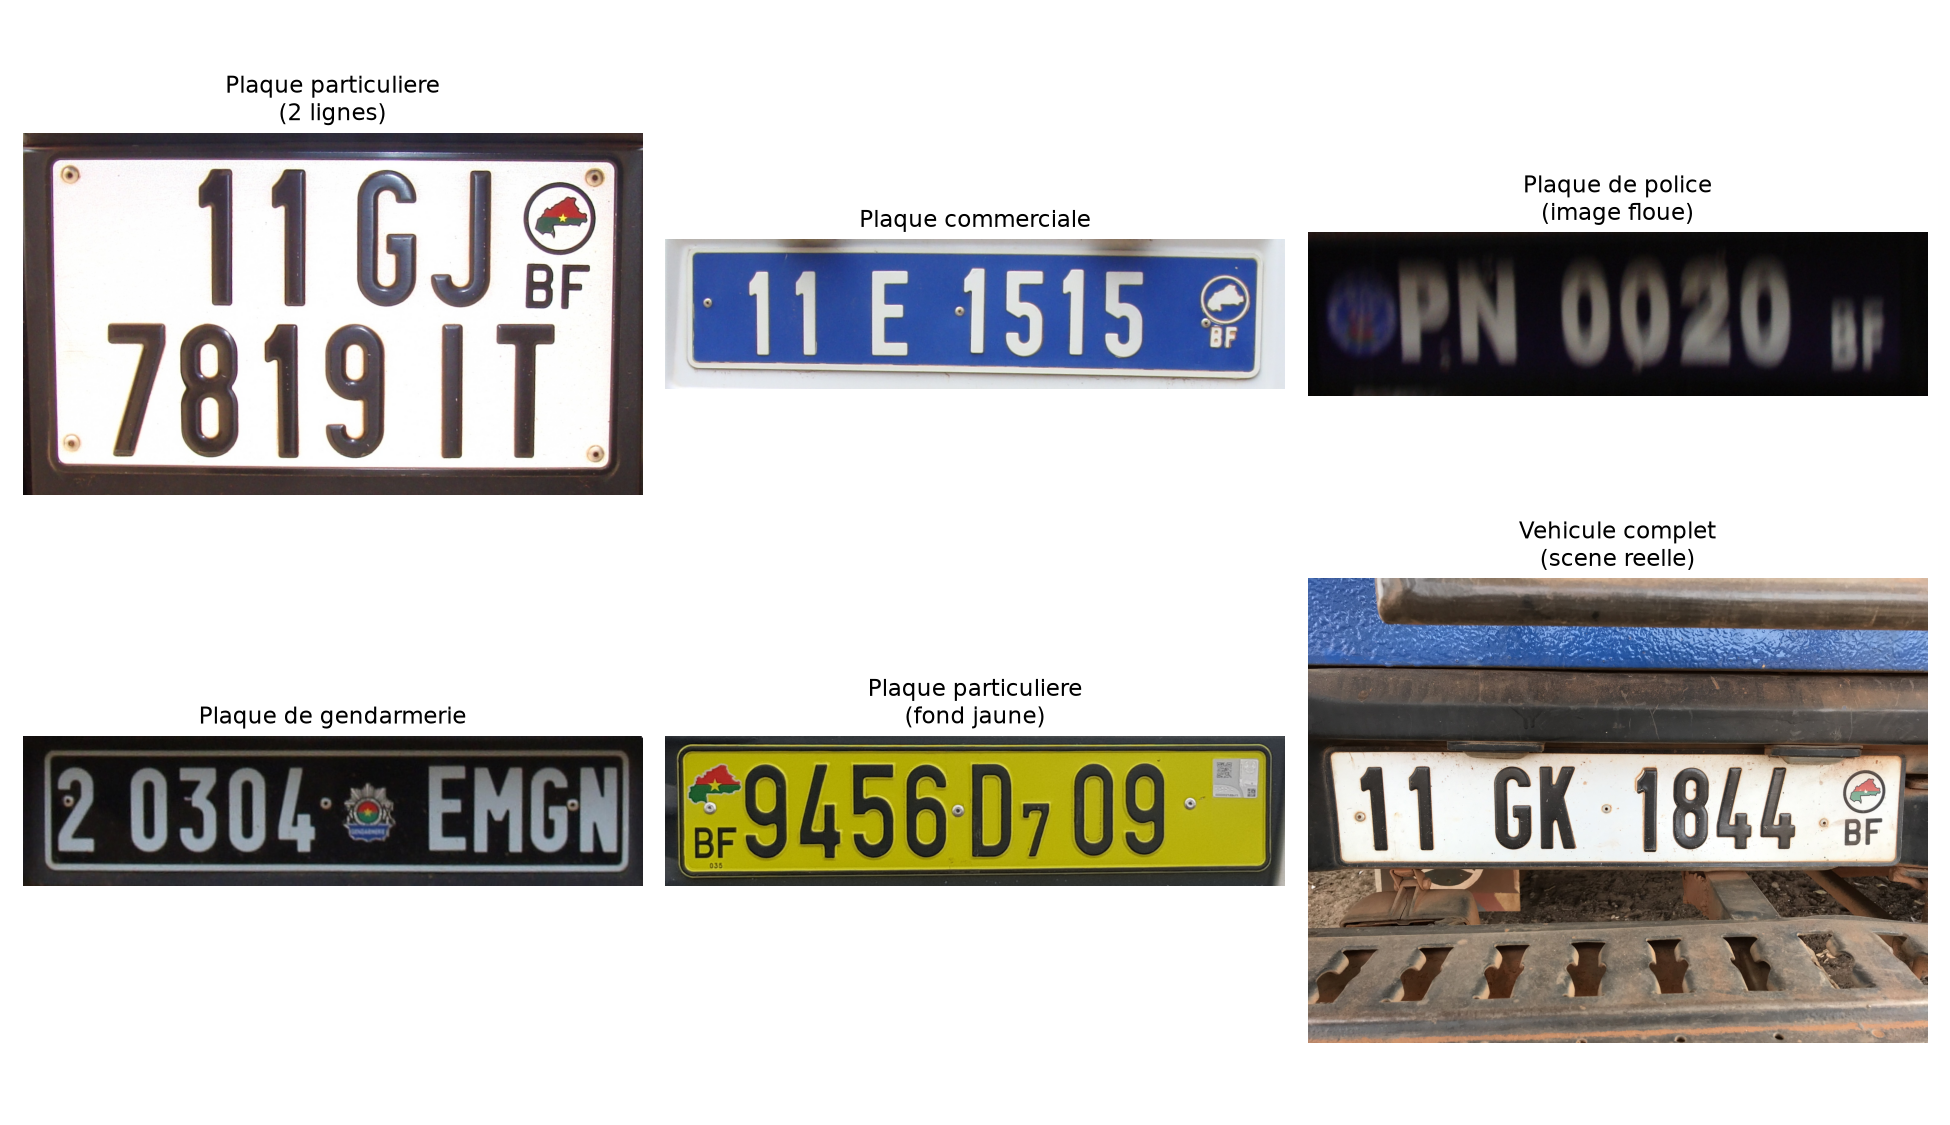
\includegraphics[width=\textwidth]{images/resultats/planche_dataset.png}
\caption{Le jeu de test documentaire~: six photographies réelles de plaques burkinabè, sous licence CC BY-SA 4.0 (Wikimedia Commons).}
\label{fig:dataset}
\end{figure}

Le second est un jeu de \textbf{photographies personnelles}~: dix-neuf photographies prises spécifiquement pour ce projet, dans des conditions réelles et variées (nuit, flash, reflets, angles de prise de vue, plaques de moto comme de voiture). Ce jeu, plus exigeant, est celui qui a le plus fait progresser l'algorithme~: chaque échec observé dessus a motivé une correction précise de la chaîne, documentée en partie~V.

Enfin, la base de \textbf{gabarits de caractères} utilisée pour la reconnaissance (section~\ref{pg:I7}) a été constituée à partir de caractères réellement segmentés sur ces deux jeux, complétée par des plaques d'un pays voisin (algériennes) extraites d'un mémoire de fin d'études sur le même sujet \cite{ref_blida}, pour enrichir la couverture de chiffres peu représentés dans nos propres photographies.

\subsection{Étape 1 --- Prétraitement}
\label{pg:I3}

La photographie d'entrée est convertie en niveaux de gris, puis lissée par un filtre bilatéral~: contrairement à un flou gaussien classique, qui moyenne indifféremment tous les pixels voisins, le filtre bilatéral ne moyenne que les pixels également proches en intensité, ce qui réduit le bruit du fond de la plaque tout en préservant les contours nets des caractères.

\subsection{Étape 2 --- Segmentation par contours~: localisation de la plaque}
\label{pg:I4}

Une plaque minéralogique concentre, sur une petite surface rectangulaire, une forte densité de contours verticaux rapprochés (les bords des caractères), nettement supérieure à celle du reste de la scène. Les points de contour sont extraits par le détecteur de Canny, qui prolonge les opérateurs de gradient (Sobel) par une suppression des non-maxima et un seuillage par hystérésis, produisant des contours plus fins et plus continus \cite{ref_canny}. Ces contours sont ensuite refermés par une fermeture morphologique (dilatation puis érosion) avec un noyau rectangulaire allongé horizontalement, qui relie entre eux les contours voisins des caractères d'une même plaque en un bloc compact.

Parmi les contours fermés obtenus, l'algorithme retient ceux dont l'aire et la forme sont compatibles avec une plaque (rapport largeur/hauteur entre 1,3 et 6,5, taux de remplissage élevé du rectangle englobant). Cette seule approche échoue cependant dès que la plaque a un fond de couleur unie mal contrasté avec son environnement, ou lorsqu'un reflet produit un gradient plus fort que celui de la plaque~: nous la complétons donc par une seconde méthode de localisation, une \textbf{segmentation par région}~: des germes répartis sur une grille régulière de l'image font croître, chacun, la région connexe des pixels dont la teinte reste proche du germe (technique de croissance de région, seuillage connecté). Les deux méthodes produisent chacune une liste de candidats~; plutôt que de figer un choix sur la seule force locale d'un contour ou d'une couleur, la localisation finale est choisie en exécutant, pour chaque candidat, la suite complète de la chaîne (redressement, binarisation, segmentation des caractères), et en retenant celui dont la segmentation obtenue est la plus plausible (section~\ref{pg:I6}). Ce principe --- générer plusieurs hypothèses et laisser le résultat final départager --- est réutilisé pour la binarisation (section~\ref{pg:I5}).

Une photographie n'est pas toujours prise bien de face~: un angle de prise de vue incline la plaque dans l'image. Nous corrigeons cette inclinaison à partir du rectangle \emph{orienté} de surface minimale englobant le contour retenu (\texttt{cv2.minAreaRect}), dont les quatre coins suivent l'inclinaison réelle de la plaque~; une transformation de perspective (\emph{four-point transform}) ramène alors ces quatre coins à un rectangle horizontal. En deçà d'un angle mesuré de 1,5~degré, l'inclinaison est jugée négligeable et un simple recadrage est conservé.

\subsection{Étape 3 --- Segmentation par région~: binarisation de la plaque}
\label{pg:I5}

Une fois la plaque extraite, elle doit être binarisée. Le seuillage global automatique par minimisation des variances (méthode d'Otsu, équivalente à la méthode de Fisher~: elle minimise la variance intra-classe entre pixels de fond et de caractères \cite{ref_otsu}) suppose un histogramme bimodal net, donc un éclairage à peu près uniforme sur la plaque~; le seuillage adaptatif, qui calcule un seuil propre à chaque voisinage, tolère un éclairage inégal mais peut fragmenter un trait par ailleurs uniforme. À cela s'ajoute la question de la polarité (caractères clairs sur fond sombre, ou l'inverse), qu'une règle de proportion de pixels ne résout pas de façon fiable dès que cette proportion approche 50~\%.

Plutôt que de figer un choix, nous générons quatre binarisations candidates (Otsu et seuillage adaptatif, chacun dans les deux polarités), et laissons l'étape suivante --- la segmentation en caractères --- départager ces candidates par la plausibilité du résultat qu'elles produisent.

\begin{figure}[H]
\centering
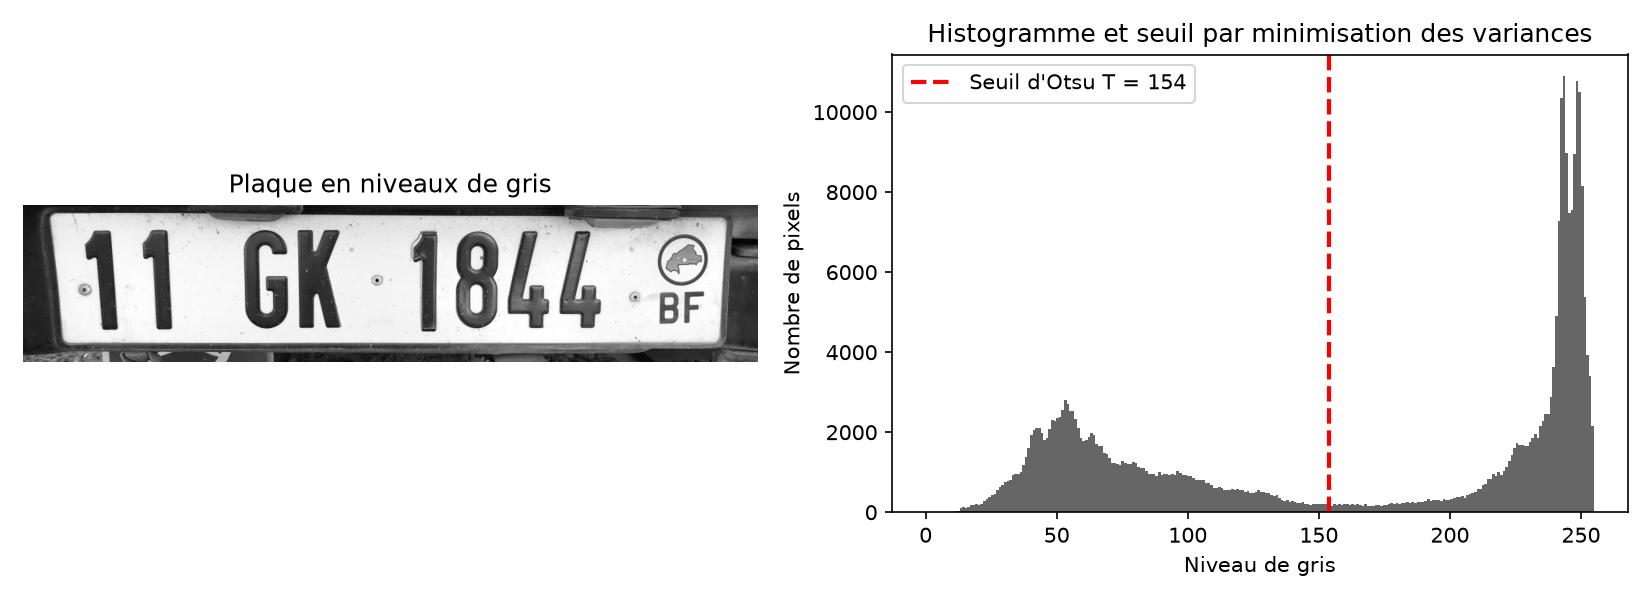
\includegraphics[width=0.85\textwidth]{images/resultats/otsu_histogramme.png}
\caption{Illustration du seuillage automatique par minimisation des variances~: l'histogramme des niveaux de gris est nettement bimodal, et le seuil d'Otsu se place dans la vallée qui sépare les deux modes.}
\label{fig:otsu}
\end{figure}

\subsection{Étape 4 --- Segmentation des caractères}
\label{pg:I6}

Chaque caractère d'une plaque binarisée est isolé par une analyse en composantes connexes~: une version systématisée de l'approche par croissance de région (agréger tous les pixels de premier plan connexes à un pixel de départ), appliquée simultanément à toute l'image. Les composantes touchant le bord du recadrage et trop grandes (cadre métallique, ou fond entier de la plaque si la polarité candidate est erronée) sont écartées, de même que celles dont la forme est incompatible avec un caractère isolé.

Un problème propre aux plaques burkinabè~: l'emblème national et le sigle \og{}BF\fg{}, empilés à gauche du numéro, se retrouvent parfois reliés par quelques pixels au premier caractère du numéro, formant une composante anormalement large. Nous la découpons par projection verticale (compter, colonne par colonne, les pixels de premier plan~: une vallée nette signale la frontière entre deux symboles), restreinte à la bande centrale de la plaque~: l'emblème et le sigle, empilés verticalement, laissent cette bande vide, alors qu'un caractère la traverse toujours.

Les composantes obtenues sont enfin filtrées par leur hauteur~: nous calculons la hauteur \emph{médiane} du groupe et ne retenons que celles qui s'en écartent de moins de 60~\%, ainsi que par leur position verticale (un élément décoratif peut avoir une hauteur plausible sans être assis sur la même ligne de base que les vrais caractères). Les caractères retenus sont regroupés par ligne (centres verticaux proches) puis ordonnés de gauche à droite~; le nombre de lignes obtenu indique directement si la plaque est écrite sur une ou deux lignes, sans que l'utilisateur ait à le préciser.

C'est cette segmentation qui permet de choisir la meilleure binarisation et la meilleure localisation (sections~\ref{pg:I4} et~\ref{pg:I5})~: un score de plausibilité combine le nombre de caractères obtenus (plausible entre 5 et 10) et l'homogénéité de leur hauteur --- des caractères gravés au même gabarit ont, par construction, des hauteurs régulières, contrairement aux artefacts de binarisation.

\subsection{Étape 5 --- Reconnaissance des caractères par comparaison de motifs}
\label{pg:I7}

C'est ici que se distingue une reconnaissance analytique, où chaque motif isolé est caractérisé puis classé indépendamment, d'une reconnaissance qui s'appuierait sur le contenu global de l'image. Conformément à la consigne du cours --- écrire nous-mêmes la logique de reconnaissance plutôt que de la confier à un outil externe --- nous retenons une reconnaissance analytique par \textbf{comparaison directe à une base de gabarits réels}~: chaque caractère segmenté est comparé, un par un, à tous les échantillons disponibles pour chaque lettre et chiffre de l'alphabet, et le caractère dont le meilleur échantillon obtient le score le plus élevé est retenu.

La mesure de similarité employée est la \textbf{mesure de similarité complémentaire} (CSM), telle que décrite dans un mémoire de fin d'études consacré au même problème \cite{ref_blida}~: pour deux images binaires $F$ (le caractère segmenté) et $T$ (le gabarit), de même taille et comptant $n$~pixels, on note $a$ le nombre de pixels noirs communs aux deux images, $b$ le nombre de pixels noirs chez $T$ seul, $c$ le nombre de pixels noirs chez $F$ seul, $e$ le nombre de pixels blancs communs, et $T_{\text{noir}} = a+b$ le nombre total de pixels noirs du gabarit. Le rapport de similarité retenu est
\[
R(F,T) = \frac{a \cdot e - b \cdot c}{T_{\text{noir}} \cdot (n - T_{\text{noir}})} \in [-1,\,1].
\]
Un rapport proche de 1 signale une forte ressemblance~; un caractère dont le meilleur rapport, tous gabarits confondus, reste sous un seuil de confiance est renvoyé comme non reconnu (\og{}?\fg{}) plutôt que comme une réponse hasardeuse.

Cette approche a été préférée à une comparaison contre des caractères générés par une police d'ordinateur~: un essai initial, avec des gabarits produits par une police vectorielle courante, a échoué de façon nette --- un \og{}8\fg{} réellement photographié y ressemblait moins à son propre gabarit qu'à un \og{}H\fg{}, le tracé embouti et photographié d'un caractère de plaque ne correspondant pas à une police vectorielle. Des gabarits constitués d'échantillons réellement photographiés et segmentés, même peu nombreux, se sont montrés nettement plus fiables (section~\ref{pg:IV3}).

% ============================================================
\section{Choix technologiques}
\label{pg:II}

\subsection{Python comme langage d'implémentation}
\label{pg:II1}

Python a été retenu pour l'ensemble de la chaîne. L'écosystème de bibliothèques de traitement d'image y est mature et accessible~: OpenCV, la bibliothèque de référence du domaine, y expose la quasi-totalité de ses fonctions avec une interface simple. Python permet un prototypage rapide~: chaque étape de la chaîne a pu être développée et visualisée indépendamment avant d'être assemblée. Une alternative telle que MATLAB aurait été envisageable, mais nous avons préféré Python pour sa gratuité et sa plus large diffusion en dehors du monde académique.

\subsection{OpenCV pour le traitement d'image}
\label{pg:II2}

L'ensemble des étapes de prétraitement, de détection de contours, de morphologie mathématique, de seuillage et d'analyse de composantes connexes repose sur OpenCV (\texttt{opencv-python}), bibliothèque libre qui implémente de façon optimisée la quasi-totalité des opérateurs classiques du cours~: filtres de convolution, opérateurs de gradient, morphologie mathématique, seuillage d'Otsu, extraction de contours et de composantes connexes \cite{ref_opencv}. Le recours à une bibliothèque unique et bien établie garantit la correction et la performance du code, et permet de concentrer l'effort sur l'assemblage et le paramétrage de la chaîne plutôt que sur la ré-implémentation d'opérateurs déjà bien connus --- ce qui reste conforme à la consigne du cours, qui autorise l'usage de bibliothèques pour les opérations de traitement d'image tant que la logique de reconnaissance elle-même est écrite par nos soins.

\subsection{Comparaison de motifs plutôt qu'un moteur de reconnaissance externe}
\label{pg:II3}

Pour la dernière étape, la reconnaissance des caractères, plusieurs pistes ont été envisagées puis écartées. Un moteur de reconnaissance optique de caractères externe (Tesseract, notamment) a été utilisé dans une version antérieure de ce projet~; il a été retiré~: la consigne du cours est d'écrire nous-mêmes l'algorithme de reconnaissance en nous appuyant sur les techniques vues en cours, pas de déléguer cette décision à un moteur tiers déjà entraîné sur d'immenses corpus de texte imprimé, dont le fonctionnement interne échappe largement à ce que nous avons pu mettre en œuvre nous-mêmes. Entraîner un classifieur appris (un petit réseau convolutif) aurait par ailleurs exigé un jeu d'entraînement de caractères annotés hors de portée du temps imparti, et nous aurait éloignés du traitement d'image classique visé par le cours.

Nous avons donc retenu la comparaison directe de motifs contre une base de gabarits réels (section~\ref{pg:I7}), au moyen de la mesure de similarité complémentaire décrite dans le mémoire de Benachour et Anede \cite{ref_blida}, que nous implémentons nous-mêmes avec NumPy~: c'est une reconnaissance analytique de primitives au sens strict du cours, entièrement interprétable, et dont chaque étape est vérifiable dans le code source.

\subsection{Synthèse des choix technologiques}
\label{pg:II4}

\begin{table}[H]
\centering
\footnotesize
\begin{tabularx}{\textwidth}{@{}L{2.9cm} L{3.6cm} X@{}}
\toprule
\textbf{Composant} & \textbf{Choix retenu} & \textbf{Justification principale}\\
\midrule
Langage & Python 3 & Écosystème de vision par ordinateur mature, prototypage rapide, gratuit.\\
Traitement d'image & OpenCV (\texttt{opencv-python}) & Implémentation optimisée et fiable des opérateurs classiques du cours.\\
Reconnaissance des caractères & Comparaison de motifs (mesure CSM), base de gabarits réels & Algorithme écrit par nos soins, conforme à la consigne du cours~; aucun moteur externe, aucun modèle appris.\\
Interface & Streamlit & Application web locale, sans configuration serveur.\\
\bottomrule
\end{tabularx}
\caption{Synthèse des choix technologiques et de leur justification}
\end{table}

% ============================================================
\section{Implémentation}
\label{pg:III}

\subsection{Organisation du code}
\label{pg:III0}

Le code source est volontairement réduit à deux fichiers, pour rester simple à lire et à vérifier~:

\begin{itemize}
\item \texttt{anpr\_pipeline.py} --- le module unique qui implémente chacune des cinq étapes décrites en partie~I, sous la forme de fonctions courtes et indépendantes, ainsi qu'une fonction \texttt{executer\_pipeline\_image} qui les enchaîne~;
\item \texttt{app.py} --- l'interface utilisateur interactive (Streamlit), présentée en section~\ref{pg:III4}, qui ne fait qu'appeler les fonctions du module précédent.
\end{itemize}

La base de gabarits de caractères (section~\ref{pg:I7}) est un dossier de données, \texttt{images/gabarits/}, contenant un sous-dossier par caractère (\texttt{0}, \texttt{1}, \ldots, \texttt{Z}) rempli d'images réellement segmentées~; elle est lue directement par \texttt{anpr\_pipeline.py} et ne dépend d'aucun script de construction supplémentaire.

\subsection{Localisation de la plaque}
\label{pg:III1}

L'extrait suivant montre les étapes~1 et~2 (prétraitement, détection des contours, candidats de localisation par contour et par région de couleur).

\begin{lstlisting}
def pretraiter(image_bgr):
    gris = cv2.cvtColor(image_bgr, cv2.COLOR_BGR2GRAY)
    gris_lisse = cv2.bilateralFilter(gris, d=9, sigmaColor=75, sigmaSpace=75)
    return gris, gris_lisse


def detecter_contours(gris_lisse):
    contours_bruts = cv2.Canny(gris_lisse, 50, 150)
    noyau = cv2.getStructuringElement(cv2.MORPH_RECT, (25, 9))
    contours_fermes = cv2.morphologyEx(contours_bruts, cv2.MORPH_CLOSE, noyau)
    return contours_bruts, contours_fermes


def candidats_par_couleur(image_bgr, aire_image, pas_grille=40, tolerance=(12, 50, 50)):
    # germes repartis sur une grille ; croissance de region par cv2.floodFill
    # (voir code source complet : anpr_pipeline.py)
    ...


def choisir_localisation(image_bgr, candidats):
    meilleur = None
    for _score_brut, boite, contour in candidats:
        plaque_couleur = extraire_plaque_redressee(image_bgr, boite, contour)
        plaque_gris = cv2.cvtColor(plaque_couleur, cv2.COLOR_BGR2GRAY)
        binaire, boites, nb_lignes, methode = segmenter_plaque(plaque_gris)
        score = _score_segmentation(grouper_en_lignes(boites))
        if meilleur is None or score > meilleur[0]:
            meilleur = (score, boite, plaque_couleur, binaire, boites, nb_lignes, methode)
    if meilleur is not None and meilleur[0] > 0:
        return meilleur[1:]
    return ...  # repli sur l'image entiere
\end{lstlisting}

\texttt{choisir\_localisation} exécute, pour chaque candidat (contour ou région de couleur), la suite complète de la chaîne, et retient celui dont la segmentation obtenue est la plus plausible.

\subsection{Binarisation, segmentation des caractères et reconnaissance}
\label{pg:III2}

\texttt{segmenter\_plaque} est la fonction charnière de la chaîne~: elle évalue chacune des quatre binarisations candidates par la plausibilité de la segmentation qu'elle produit, et ne retient que la meilleure.

\begin{lstlisting}
def segmenter_plaque(plaque_gris):
    meilleure = None
    for nom, binaire in variantes_binarisation(plaque_gris):
        boites = _composantes_brutes(binaire)
        boites = _separer_composantes_larges(binaire, boites)
        boites = _filtrer_forme_caractere(boites)
        boites = _retenir_caracteres_coherents(boites)
        lignes = grouper_en_lignes(boites)
        score = _score_segmentation(lignes)
        if meilleure is None or score > meilleure[0]:
            meilleure = (score, nom, binaire, lignes)
    score, nom, binaire, lignes = meilleure
    boites_ordonnees = [b for ligne in lignes for b in ligne]
    return binaire, boites_ordonnees, len(lignes), nom
\end{lstlisting}

La reconnaissance (section~\ref{pg:I7}) est implémentée par les deux fonctions suivantes~: \texttt{\_similarite\_csm} calcule le rapport de similarité entre un caractère segmenté et un gabarit, et \texttt{detailer\_reconnaissance} compare chaque caractère à toute la base pour retenir le meilleur.

\begin{lstlisting}
def _similarite_csm(vignette, gabarit):
    f = vignette > 127
    t = gabarit > 127
    a = int(np.count_nonzero(f & t))
    b = int(np.count_nonzero(~f & t))
    c = int(np.count_nonzero(f & ~t))
    e = int(np.count_nonzero(~f & ~t))
    n = f.size
    T = a + b
    denominateur = T * (n - T)
    return (a * e - b * c) / denominateur if denominateur else 0.0


def detailer_reconnaissance(binaire, boites, marge=4, seuil_confiance=0.2):
    details = []
    for (x, y, w, h) in boites:
        vignette = ...  # vignette recadree et redimensionnee
        meilleur_c, meilleur_score = "?", seuil_confiance
        for c, echantillons in _gabarits_caracteres.items():
            for gabarit in echantillons:
                score = _similarite_csm(vignette, gabarit)
                if score > meilleur_score:
                    meilleur_score, meilleur_c = score, c
        details.append({"vignette": vignette, "caractere": meilleur_c, "score": meilleur_score})
    return details
\end{lstlisting}

Le code source complet, avec l'ensemble des fonctions intermédiaires et leurs commentaires, est fourni dans \texttt{code/anpr\_pipeline.py}.

\subsection{Interface utilisateur interactive}
\label{pg:III4}

\begin{figure}[H]
\centering
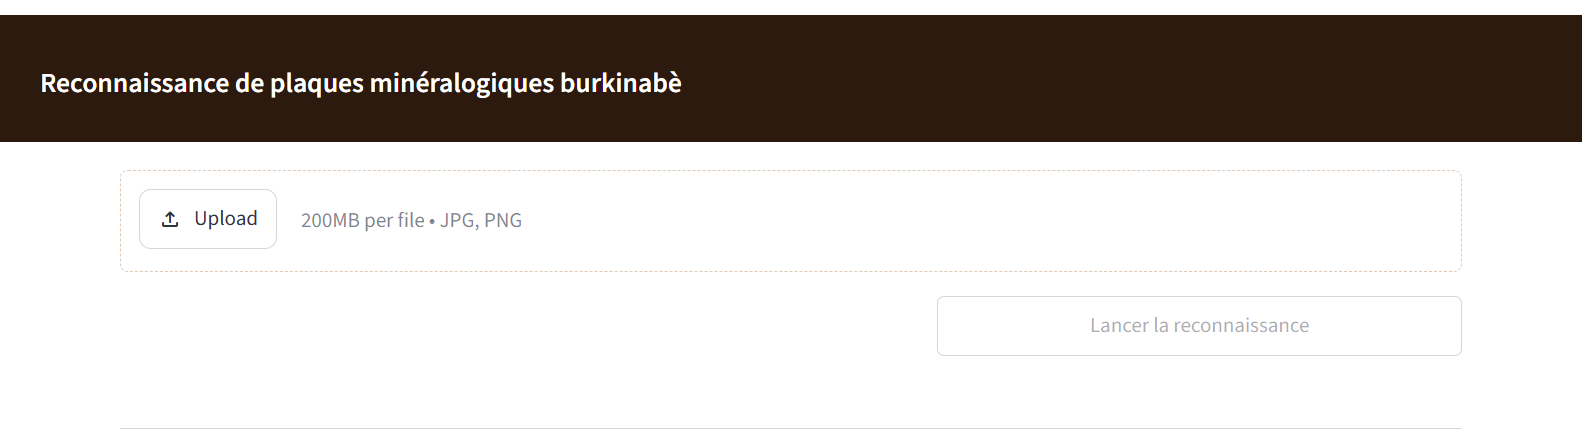
\includegraphics[width=0.78\textwidth]{images/captures_app/1_accueil_explication.png}
\caption{Capture d'écran de l'application au démarrage~: une seule zone de dépôt de photographie, aucun réglage technique à renseigner.}
\label{fig:interface_accueil}
\end{figure}

L'ensemble de la chaîne est enveloppé dans une application web interactive construite avec Streamlit (\texttt{code/app.py}), lancée localement par la commande \texttt{streamlit run app.py}. L'utilisateur y dépose une photographie~; l'application affiche successivement les huit images correspondant à chacune des étapes de traitement (prétraitement, contours, fermeture morphologique, localisation, plaque extraite, binarisation, segmentation), puis une neuvième étape qui montre, caractère par caractère, la vignette segmentée, le gabarit le plus proche retenu et le score de similarité obtenu --- rendant visible, pour chaque caractère, la décision prise par la comparaison de motifs. Une carte de résultat affiche enfin le texte reconnu.

Aucun réglage technique n'est demandé à l'utilisateur~: le nombre de lignes de la plaque, la méthode de binarisation et la méthode de localisation sont déterminés automatiquement. Chaque photographie déposée est conservée (dossier \texttt{images/televerses/}), ce qui a permis, tout au long du projet, de diagnostiquer et de corriger la chaîne sur des cas réels.

\begin{figure}[H]
\centering
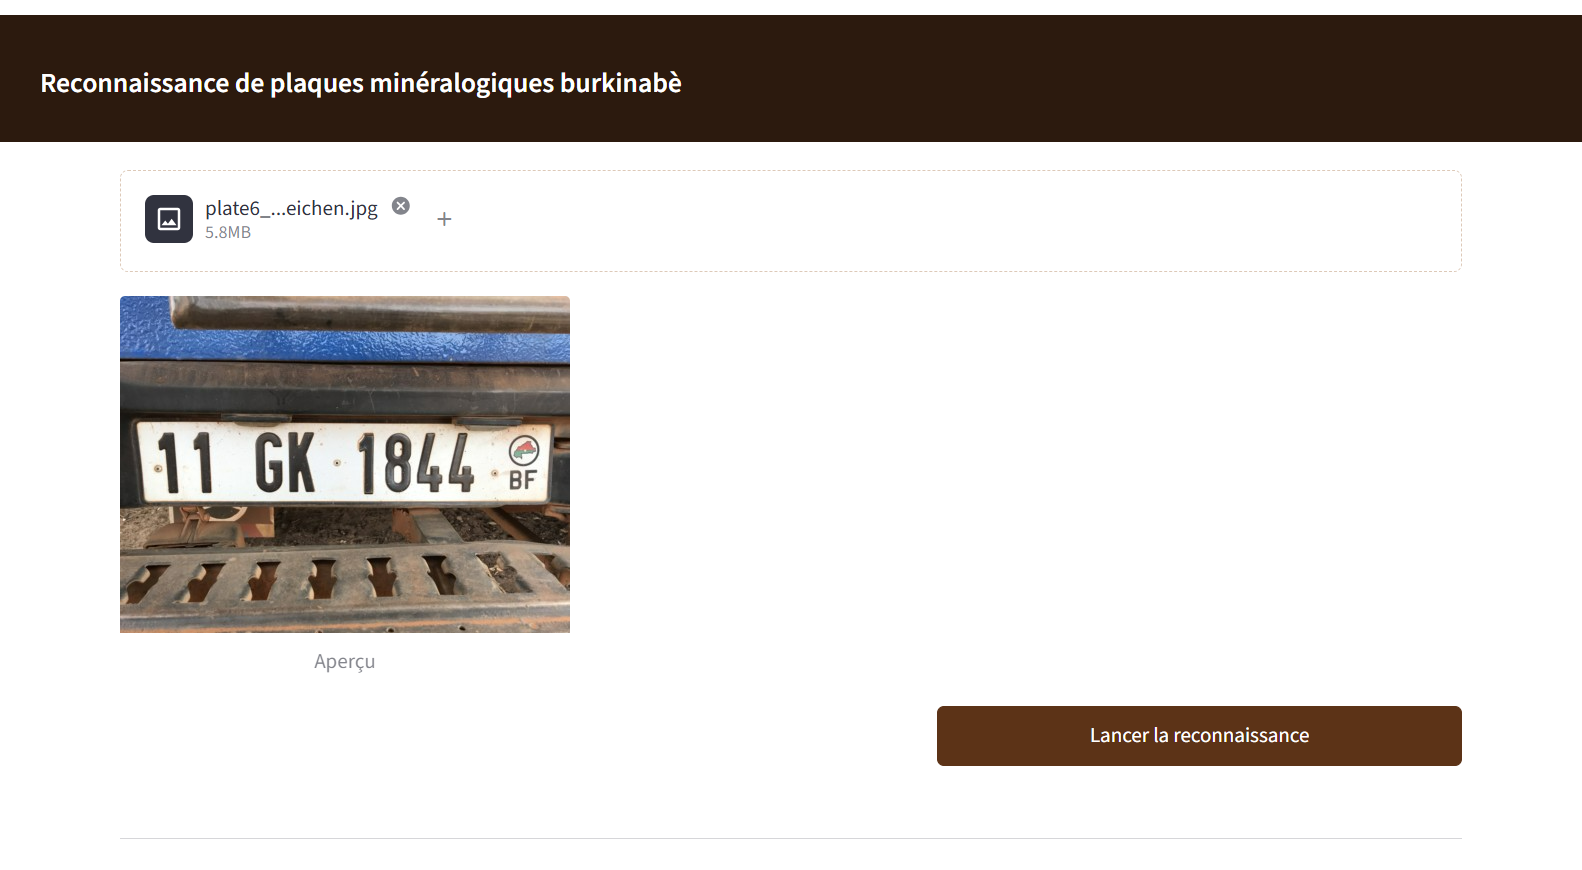
\includegraphics[width=0.78\textwidth]{images/captures_app/2_plaque_selectionnee.png}
\caption{Capture d'écran de l'application~: une photographie a été déposée, son aperçu s'affiche, prête pour le lancement de la reconnaissance.}
\label{fig:interface_apercu}
\end{figure}

% ============================================================
\section{Résultats}
\label{pg:IV}

\subsection{Jeu de test documentaire}
\label{pg:IV1}

\begin{table}[H]
\centering
\footnotesize
\begin{tabularx}{\textwidth}{@{}C{0.9cm} L{3.4cm} L{3.4cm} X@{}}
\toprule
\textbf{N°} & \textbf{Image} & \textbf{Format} & \textbf{Vérité terrain}\\
\midrule
1 & plate1\_passenger & Particulière, 2 lignes & 11GJ7819IT\\
2 & plate2\_commercial & Commerciale (fond bleu) & 11E1515\\
3 & plate3\_police & Police (image floue) & PN0020\\
4 & plate4\_gendarmerie & Gendarmerie (fond noir) & 20304EMGN\\
5 & plate5\_kennzeichen301 & Particulière (fond jaune) & 9456D709\\
6 & plate6\_kennzeichen & Véhicule complet (scène réelle) & 11GK1844\\
\bottomrule
\end{tabularx}
\caption{Jeu de test documentaire~: six plaques burkinabè et leur vérité terrain}
\label{tab:jeu_test}
\end{table}

\subsection{Résultats sur le jeu documentaire}
\label{pg:IV3}

\begin{table}[H]
\centering
\small
\begin{tabularx}{\textwidth}{@{}C{0.9cm} L{2.6cm} L{2.6cm} C{2cm} X@{}}
\toprule
\textbf{Plaque} & \textbf{Vérité terrain} & \textbf{Reconnu} & \textbf{Similarité} & \textbf{Remarque}\\
\midrule
1 & 11GJ7819IT & 11GJ7819IT & \textbf{100\,\%} & exact\\
2 & 11E1515 & 11E1818 & 71\,\% & deux caractères confondus (5$\to$8, 5$\to$8)\\
3 & PN0020 & IN00I0 & 67\,\% & photo très floue, base de gabarits sans \og{}P\fg{}\\
4 & 20304EMGN & 20304EMGN & \textbf{100\,\%} & exact\\
5 & 9456D709 & 9488D09 & 62\,\% & \og{}7\fg{} en indice non segmenté, un caractère confondu\\
6 & 11GK1844 & 11GK1844 & \textbf{100\,\%} & exact\\
\midrule
\multicolumn{3}{@{}l}{\textbf{Moyenne}} & \textbf{83\,\%} &\\
\bottomrule
\end{tabularx}
\caption{Résultats de reconnaissance par comparaison de motifs sur le jeu documentaire}
\label{tab:resultats}
\end{table}

Trois plaques sur six sont reconnues exactement. Les trois autres illustrent chacune une limite précise, discutée en partie~V~: confusion entre deux chiffres de forme proche dans la base de gabarits (2), photo trop dégradée combinée à une base encore incomplète (3), et petit caractère en indice non segmenté (5).

\begin{figure}[H]
\centering
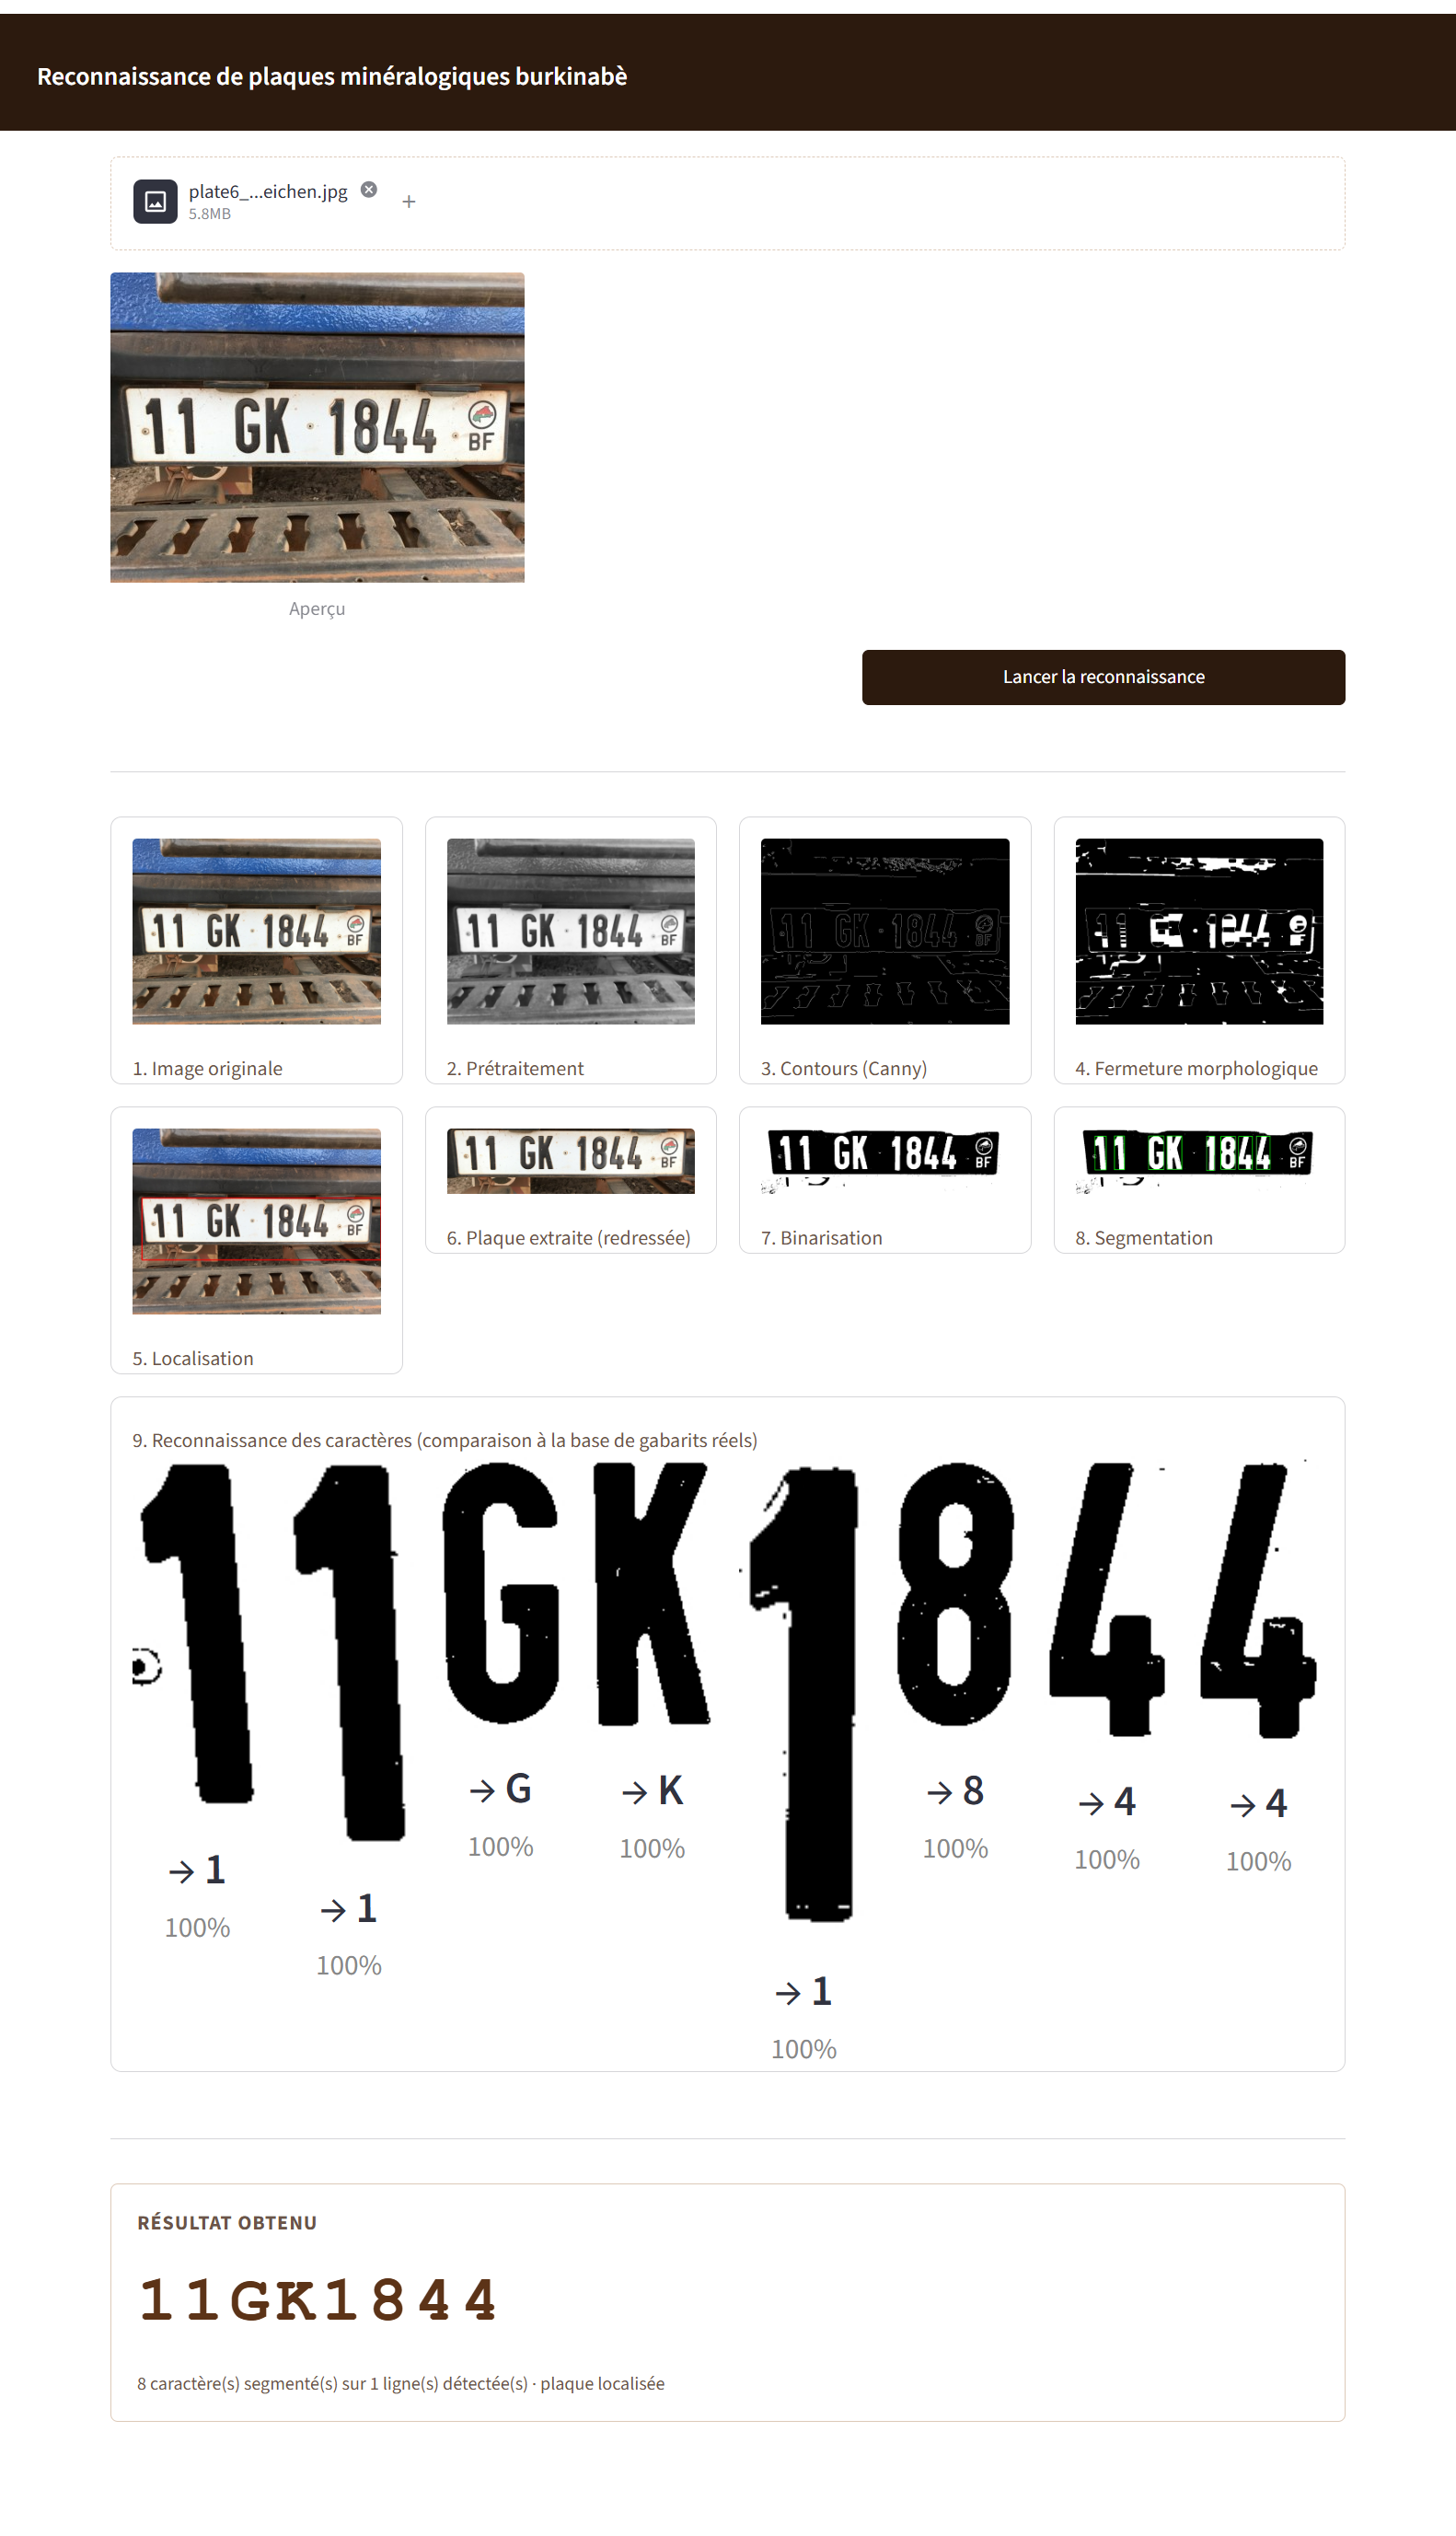
\includegraphics[width=0.62\textwidth]{images/captures_app/3_resultats_completes.png}
\caption{Capture d'écran de l'application sur \texttt{plate6\_kennzeichen}, seule photographie du jeu documentaire montrant un véhicule entier~: les neuf étapes s'enchaînent jusqu'à la comparaison caractère par caractère avec la base de gabarits, pour un résultat exact (\og{}11GK1844\fg{}).}
\label{fig:etapes_succes}
\end{figure}

\begin{figure}[H]
\centering
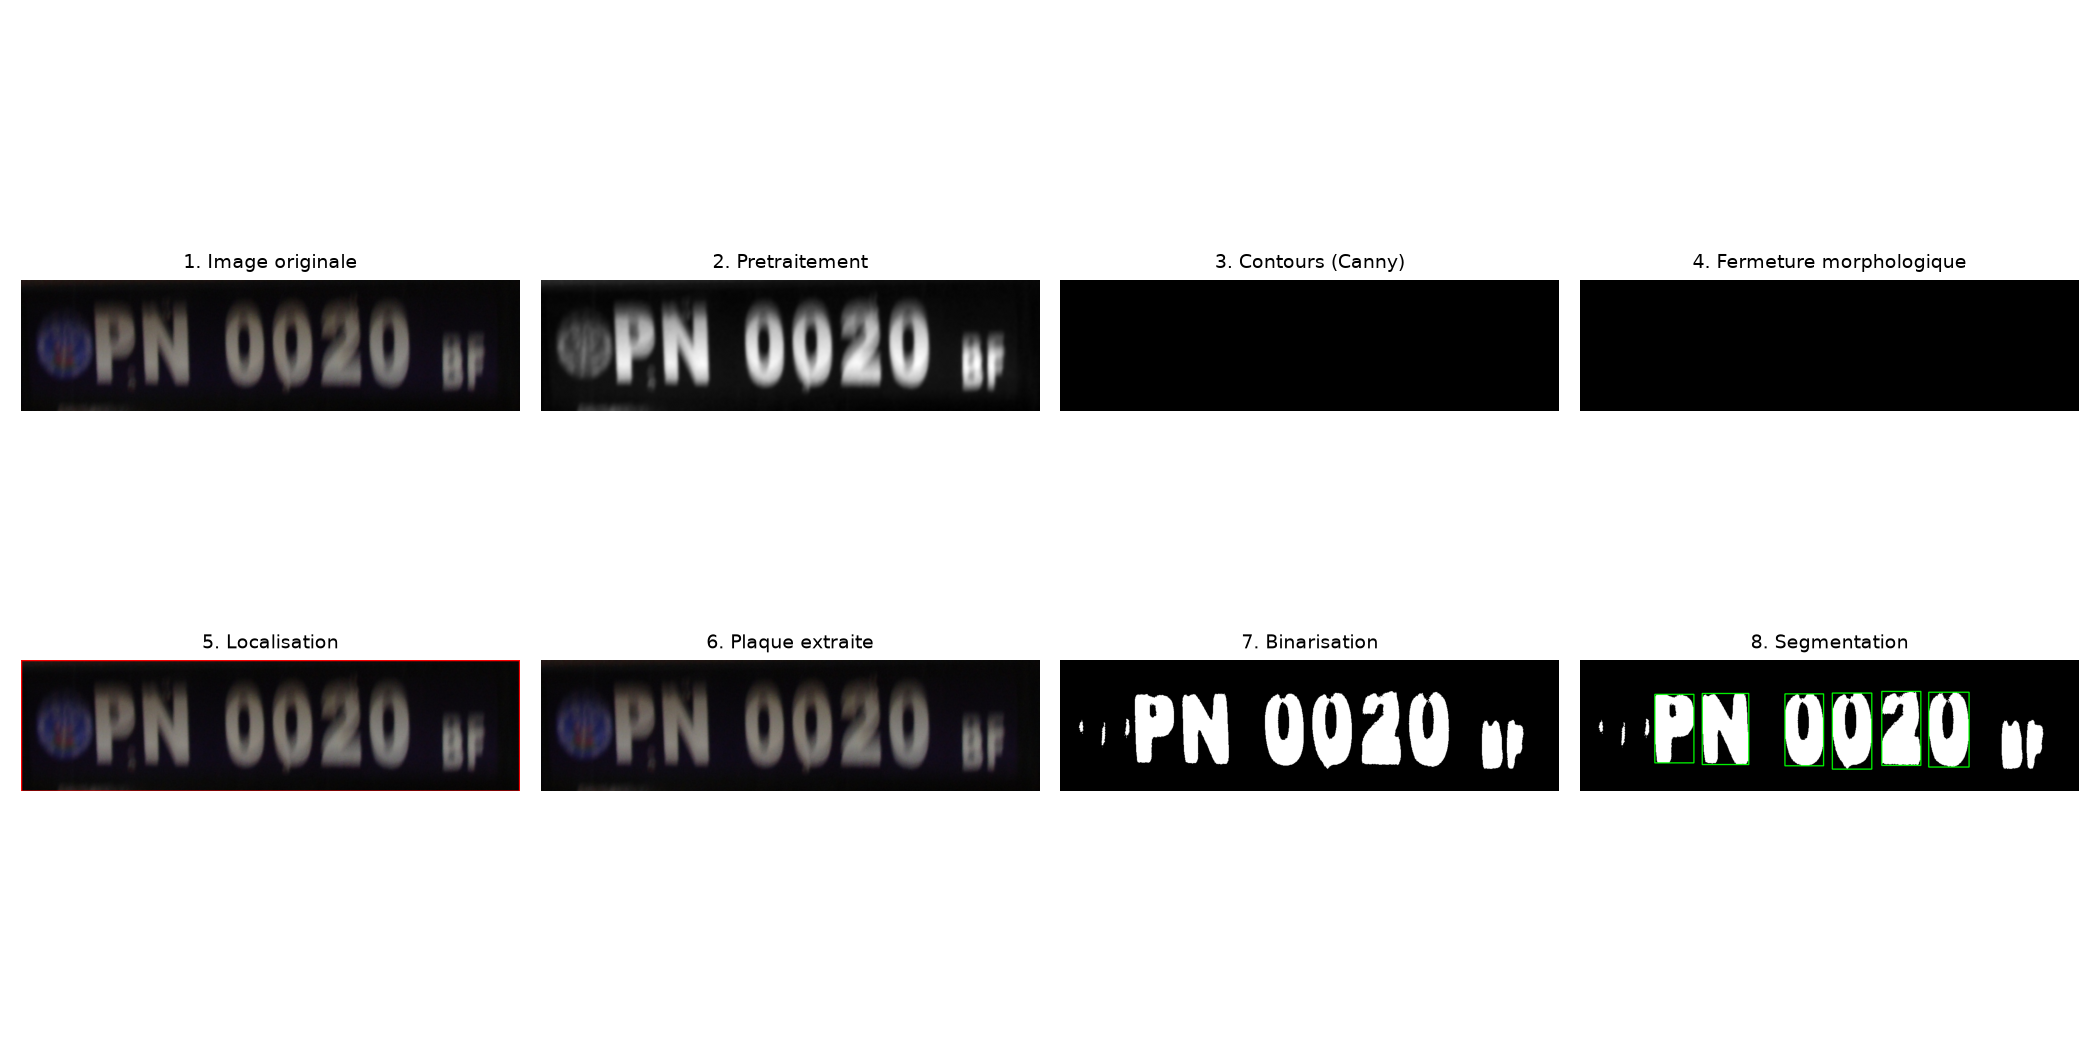
\includegraphics[width=\textwidth]{images/resultats/plate3_police_etapes.png}
\caption{Chaîne complète sur \texttt{plate3\_police}, photographie fortement affectée par un flou de mouvement~: le détecteur de Canny ne trouve quasiment aucun contour exploitable, mais la binarisation reste suffisamment lisible pour une reconnaissance partielle.}
\label{fig:etapes_flou}
\end{figure}

\subsection{Résultats sur des photographies personnelles}
\label{pg:IV4}

Un second jeu, plus exigeant, a été constitué~: dix-neuf photographies personnelles, prises en conditions réelles (nuit, flash, angles variés, plaques de moto et de voiture). À la manière du mémoire de référence que nous citons en bibliographie \cite{ref_blida}, qui présente séparément les plaques reconnues et non reconnues de son propre jeu de test, nous présentons ici quelques cas représentatifs plutôt que la liste exhaustive, disponible dans \texttt{images/resultats/resultats\_reels.csv}.

\textbf{Succès complets.} Deux photographies sont reconnues exactement~: une plaque de moto à fond jaune (\og{}9938 8DE03\fg{}) et une autre plaque de moto (\og{}3014 1E03\fg{}), toutes deux correspondant à des caractères déjà bien représentés dans la base de gabarits.

\begin{figure}[H]
\centering
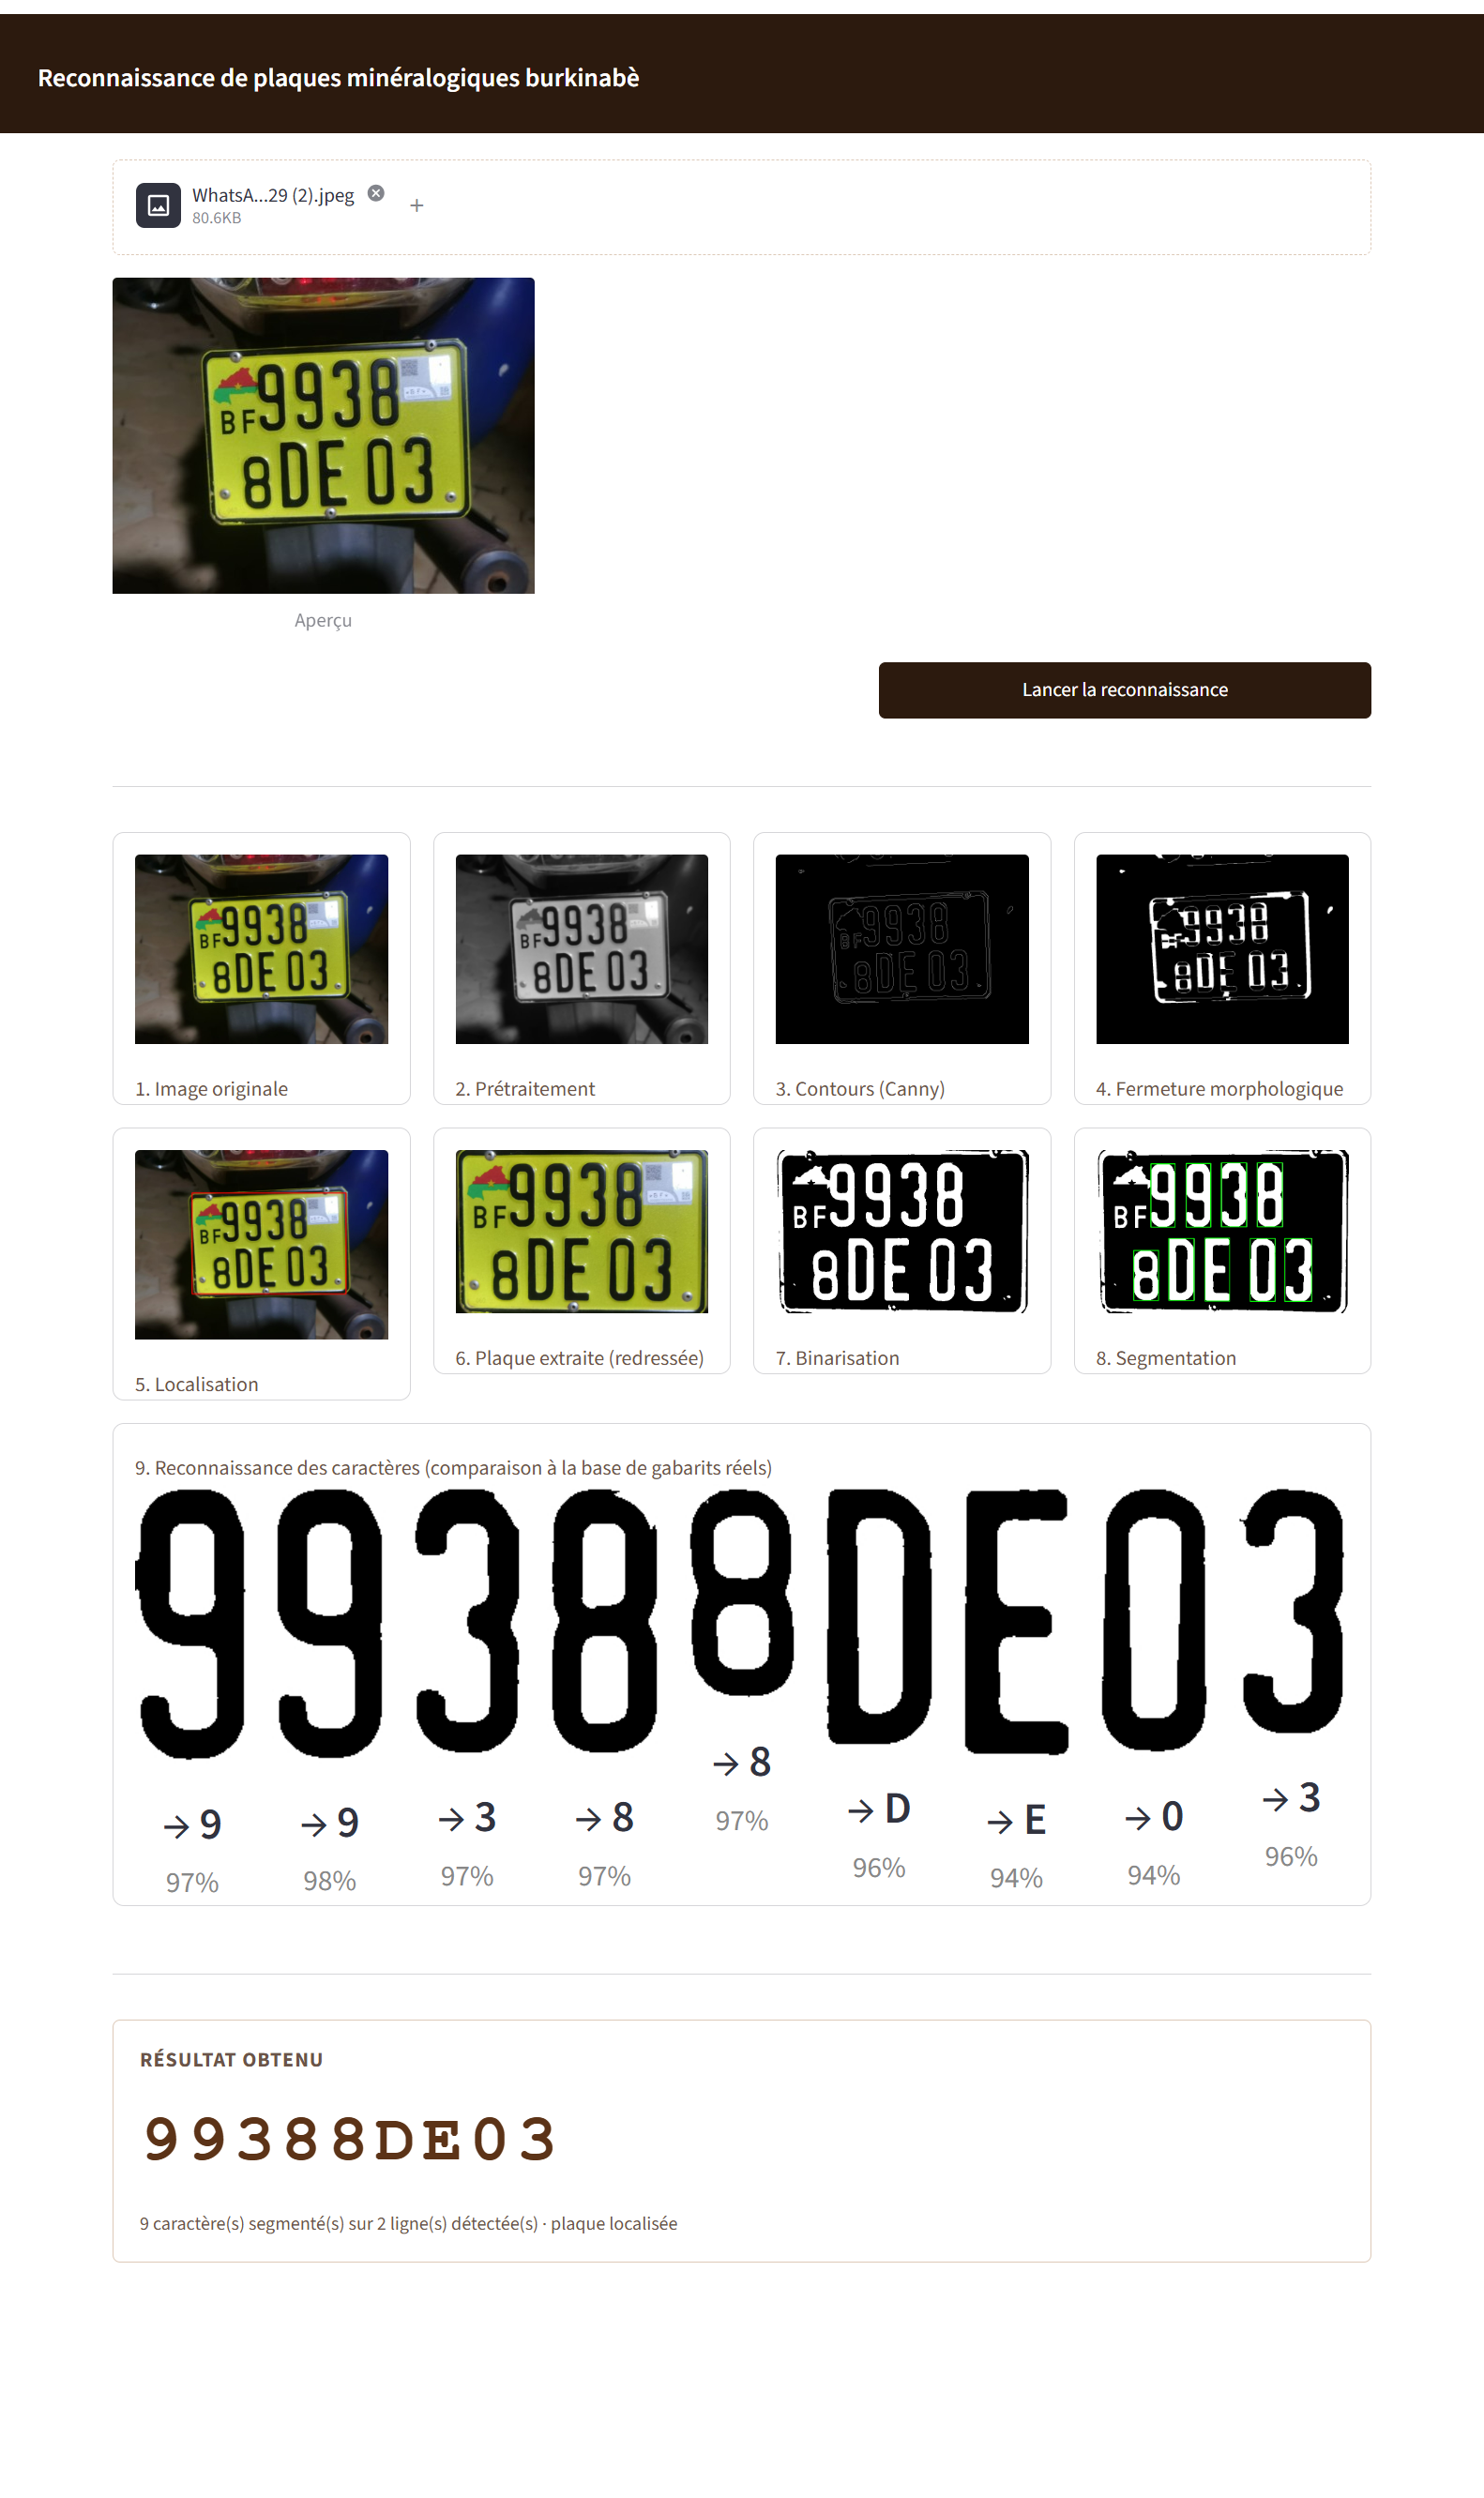
\includegraphics[width=0.62\textwidth]{images/captures_app/4_resultat_photo_reelle.png}
\caption{Capture d'écran de l'application sur une photographie personnelle (plaque de moto à fond jaune)~: malgré un reflet du flash sur la plaque, les neuf caractères sont segmentés et reconnus exactement (\og{}99388DE03\fg{}).}
\label{fig:resultat_reel_succes}
\end{figure}

\textbf{Succès partiels.} Sur une plaque \og{}9984 E3 03\fg{} photographiée de nuit au flash, la chaîne reconnaît \og{}0084E03\fg{}~: la localisation et la segmentation réussissent, mais les deux \og{}9\fg{} sont confondus avec des \og{}0\fg{}, la base de gabarits ne comptant, au moment du test, qu'un nombre restreint d'échantillons pour ce chiffre.

\textbf{Échecs et leur cause.} Une plaque \og{}11 PQ 5397\fg{} n'est reconnue que partiellement (\og{}209391\fg{})~: le \og{}11\fg{} en début de plaque, plus petit que le reste du numéro, est fusionné à la binarisation avec le cadre physique de la plaque et n'est jamais isolé comme caractère~; les lettres \og{}P\fg{} et \og{}Q\fg{}, absentes de la base de gabarits, sont confondues avec les chiffres qui leur ressemblent le plus. Une plaque photographiée de nuit dans l'obscurité quasi totale (\og{}11 JJ 2557\fg{}) n'est pas reconnue de façon exploitable~: le contraste y est si faible que ni le détecteur de contours ni la segmentation par région ne trouvent d'information suffisante --- une limite physique de la photographie elle-même, pas un défaut de l'algorithme.

\begin{table}[H]
\centering
\footnotesize
\begin{tabularx}{\textwidth}{@{}L{6.2cm} C{1.6cm} C{1.3cm} L{5.2cm}@{}}
\toprule
\textbf{Cas} & \textbf{Reconnu} & \textbf{Lignes} & \textbf{Cause principale}\\
\midrule
9938 8DE03 (moto, flash) & 99388DE03 & 2 & succès complet\\
3014 1E03 (moto, flash) & 30141E03 & 2 & succès complet\\
9984 E3 03 (voiture, nuit) & 0084E03 & 1 & \og{}9\fg{} confondu, base restreinte\\
11 PQ 5397 (moto) & 209391 & 1 & \og{}11\fg{} fusionné au cadre~; \og{}P\fg{}, \og{}Q\fg{} absents de la base\\
11 JJ 2557 (nuit, sans flash) & \'echec & -- & contraste insuffisant sur la photo elle-même\\
\bottomrule
\end{tabularx}
\caption{Exemples représentatifs sur les photographies personnelles (jeu complet~: \texttt{images/resultats/resultats\_reels.csv})}
\label{tab:resultats_reels}
\end{table}

\subsection{Synthèse}
\label{pg:IV5}

La reconnaissance par comparaison de motifs fonctionne bien dès que le caractère à reconnaître est correctement segmenté et représenté dans la base de gabarits~: les trois plaques exactement reconnues du jeu documentaire, et les deux succès complets du jeu personnel, en témoignent. Les échecs observés relèvent presque tous d'une même cause~: une base de gabarits encore restreinte, qui ne couvre pas encore tous les chiffres et lettres avec assez d'exemples. C'est une limite de \emph{données}, pas de \emph{méthode}~: elle s'améliore mécaniquement à mesure que la base est enrichie, sans qu'il soit nécessaire de changer d'algorithme.

% ============================================================
\section{Discussion~: limites et perspectives}
\label{pg:V}

\textbf{Base de gabarits encore restreinte.} C'est la limite la plus fréquemment rencontrée dans nos tests (partie~IV)~: certains chiffres et lettres ne sont représentés que par un ou deux échantillons, parfois aucun, ce qui conduit à des confusions systématiques (un \og{}9\fg{} lu \og{}0\fg{}, un \og{}P\fg{} absent de la base et confondu avec un chiffre proche). Nous avons enrichi cette base en segmentant des caractères supplémentaires depuis des plaques algériennes présentées dans le mémoire de Benachour et Anede \cite{ref_blida}, mais elle reste, à ce stade, loin d'une couverture complète de l'alphabet~: c'est la piste d'amélioration la plus directe pour ce projet.

\textbf{Petits caractères en indice.} Plusieurs plaques burkinabè font figurer un chiffre plus petit, en indice, à côté d'une lettre (par exemple le \og{}7\fg{} de \og{}E7\fg{}, ou le \og{}11\fg{} en préfixe de certains formats). Ce caractère, plus petit que le reste du numéro, est parfois fusionné par la binarisation avec un élément voisin (le cadre de la plaque, une autre lettre) et n'est alors jamais isolé comme composante à part entière. Une tentative de récupération ciblée de ces petits caractères a été testée~: elle a amélioré certains cas mais dégradé d'autres plaques qui fonctionnaient déjà, en confondant du bruit avec un indice~; elle a donc été retirée plutôt que conservée en l'état, en attendant un critère plus robuste.

\textbf{Sensibilité au flou et à la faible luminosité.} Une détection de contours fondée sur le gradient d'intensité perd son efficacité dès que l'image est floue (\texttt{plate3\_police}, figure~\ref{fig:etapes_flou})~: c'est une limite structurelle de toute approche basée contours. De même, une photographie prise dans une obscurité quasi totale (partie~\ref{pg:IV4}) ne contient parfois tout simplement plus assez de contraste entre le caractère et son fond pour qu'aucune méthode de seuillage ne puisse les séparer~: la limite est alors dans la photographie elle-même, pas dans l'algorithme.

\textbf{Localisation~: simplicité choisie plutôt que subie.} Une version antérieure de ce projet explorait la fermeture morphologique à trois échelles différentes, pour s'adapter à une plaque grande ou petite dans le cadre. Cette complexité supplémentaire n'a pas été conservée~: elle rendait le code plus difficile à suivre sans améliorer les résultats de façon mesurable --- une seule échelle de fermeture, combinée à la segmentation par région comme méthode complémentaire de localisation (section~\ref{pg:I4}), donne des résultats au moins aussi bons. C'est un choix délibéré de ce rapport~: préférer un code simple et clair à une accumulation de cas particuliers, conformément à la consigne du cours.

\textbf{Jeux de test restreints.} Les résultats chiffrés portent sur six photographies documentaires et dix-neuf photographies personnelles~: cela illustre des phénomènes réels et reproductibles, mais ne permet pas d'estimer un taux de réussite généralisable à l'ensemble du parc automobile burkinabè. Une évaluation rigoureuse demanderait plusieurs dizaines de photographies supplémentaires, en conditions de circulation réelles.

Ces limites ouvrent des pistes concrètes~: enrichissement méthodique de la base de gabarits (c'est, de loin, le levier le plus direct), un critère plus robuste pour récupérer les petits caractères en indice sans réintroduire de bruit, et la constitution d'un jeu de photographies de rue plus large pour une évaluation statistiquement solide.

\clearpage
% ============================================================
\titrecentre{Conclusion générale}
\addcontentsline{toc}{section}{Conclusion générale}
\label{pg:conclusion}

Ce projet a décrit, implémenté et évalué une chaîne complète de reconnaissance de plaque minéralogique, appliquée aux plaques d'immatriculation burkinabè. La méthodologie retenue reste fidèle au cadre du cours \emph{Reconnaissance de motifs}~: une chaîne de traitement d'image classique et interprétable (prétraitement, segmentation par contours et par région pour la localisation et le redressement, segmentation par région pour la binarisation, composantes connexes pour la segmentation des caractères), et une reconnaissance analytique par comparaison directe de motifs --- chaque caractère segmenté contre une base de gabarits réels, au moyen d'une mesure de similarité écrite par nos soins --- plutôt qu'un moteur de reconnaissance externe.

Les résultats obtenus montrent que cette approche fonctionne~: 83~\% de similarité moyenne sur le jeu documentaire, trois plaques sur six exactement reconnues, et des succès complets sur des photographies personnelles prises dans des conditions réelles. Les échecs observés, présentés sans détour en partie~IV, relèvent presque tous d'une même cause identifiée~: une base de gabarits encore restreinte, qui ne couvre pas tout l'alphabet avec assez d'exemples. C'est une limite de données, pas de méthode~: elle est appelée à se résorber à mesure que la base s'enrichit.

Ce travail a été façonné par un usage réel~: chaque limite identifiée sur des photographies personnelles, hors du seul jeu documentaire initial, a nourri une correction précise de la chaîne --- redressement de perspective pour une plaque photographiée de biais, stratégie à quatre binarisations candidates pour une plaque dont la polarité basculait à tort, découpage géométrique pour séparer l'emblème national d'un chiffre fusionné, segmentation par région en complément des contours pour une plaque de couleur unie mal détectée par le gradient. Le choix, enfin, de retirer un moteur de reconnaissance externe au profit d'une comparaison de motifs écrite par nos soins, ainsi que la simplification du code qui a suivi, illustrent qu'un système de traitement d'image gagne, autant que possible, à rester lisible et vérifiable~: c'est ce qui permet de comprendre précisément pourquoi il réussit, et pourquoi il échoue.

\clearpage
% ============================================================
\titrecentre{Bibliographie}
\addcontentsline{toc}{section}{Bibliographie}
\label{pg:biblio}

\begin{thebibliography}{99}

\bibitem{ref_cours} J. S. D. Ouattara, \emph{Reconnaissance de motifs}, support de cours, IBAM / Université Joseph KI-ZERBO, version 2026.

\bibitem{ref_blida} S. Benachour et Y. Anede, \emph{Conception et réalisation d'un système de reconnaissance de plaque d'immatriculation de véhicules en temps réel}, mémoire de master, Université Saad Dahleb, Blida, 2015--2016.

\bibitem{ref_wiki_plaques} \emph{Vehicle registration plates of Burkina Faso}, Wikipédia. \url{https://en.wikipedia.org/wiki/Vehicle_registration_plates_of_Burkina_Faso}

\bibitem{ref1} S. Du, M. Ibrahim, M. Shehata, and W. Badawy, « Automatic License Plate Recognition (ALPR): A State-of-the-Art Review », \emph{IEEE Transactions on Circuits and Systems for Video Technology}, vol.~23, no.~2, pp.~311--325, 2013.

\bibitem{ref2} C. N. E. Anagnostopoulos, I. E. Anagnostopoulos, I. D. Psoroulas, V. Loumos, and E. Kayafas, « License Plate Recognition From Still Images and Video Sequences: A Survey », \emph{IEEE Transactions on Intelligent Transportation Systems}, vol.~9, no.~3, pp.~377--391, 2008.

\bibitem{ref_canny} J. Canny, « A Computational Approach to Edge Detection », \emph{IEEE Transactions on Pattern Analysis and Machine Intelligence}, vol.~PAMI-8, no.~6, pp.~679--698, 1986.

\bibitem{ref_otsu} N. Otsu, « A Threshold Selection Method from Gray-Level Histograms », \emph{IEEE Transactions on Systems, Man, and Cybernetics}, vol.~9, no.~1, pp.~62--66, 1979.

\bibitem{ref_opencv} G. Bradski, « The OpenCV Library », \emph{Dr. Dobb's Journal of Software Tools}, 2000. \url{https://opencv.org/}

\end{thebibliography}

\end{document}
